\section{Informatique contextuelle}
Au centre des systèmes pervasifs et de l'informatique ubiquitaire, l'informatique contextuelle se fait une part de plus en plus grande. Encore une fois, sa définition a fait l'objet de plusieurs débats au sein de la communauté scientifique. Celle la plus couramment utilisé est : << L'informatique contextuelle (\textit{context-aware computing} a pour but de permettre les équipements de fournir de meilleurs services aux utilisateurs par l'utilisation d'information de contexte >>\cite{Han:contextaware}.

\subsection{Définition et applications}
La définition de contexte a été elle aussi au cœur de nombreux débats. Après analyse des travaux sur le sujet, le rapport de recherche \cite{Dey:context} propose la définition suivante :

\begin{defi}[Contexte]
Un contexte est toute information pouvant être utilisée pour caractériser la situation d'une entité. Cette entité pouvant être une personne, un lieu, ou un objet considéré comme pertinent à l'interaction entre l'utilisateur et l'application, incluant l'utilisateur et l'applications eux-mêmes.
\end{defi}

Il est important de noter sa définition est donc orientée par l'utilisation avant tout qui en est faite. Une donnée quelconque peut être un contexte s'il est utilisé comme tel. Ainsi, il nous faut voir l'ensemble des utilisations de ce contexte. Ces applications visent sept utilisations principales~\cite{Soylu:context} : 
\begin{enumerate}
	\item Sélection et recommandations d'informations ou de services.
	\item Présentation et accès à l'information et aux services.
	\item Recherche d'information ou de service.
	\item Adaptation de l'exécution de processus séquentiels.
	\item Modification et reconfiguration d'applications.
	\item Conseil d'actions semi-automatique.
	\item Allocations de ressources.
\end{enumerate}
\TODO{Est-il nécessaire de fournir des explications ?}

Les thèmes de ces applications sont directement reliés à la supervision car c'est elle qui permet la construction de ce contexte pour ensuite fournir ces types de services de haut-niveau.

\subsection{Modélisation et capture du contexte}
Le modèle utilisé pour créer et manipuler le contexte peut être sous différentes formes : Basé sur des principes d'intelligence artificielle (ontologies, réseau bayésiens), sur le génie logiciel (UML), les bases de données (Entité-Relation) ou d'autres moyens applicatifs (entrées clefs-valeurs). L'UML et l'ER atteignent rapidement leurs limites d'expressivité. Il devient difficile de manipuler les données sémantiques dans le cadre de contextes larges et hétérogènes à cause de leur rigidité. Leurs fonctionnalités permettent d'abstraire une partie du monde ou de la logique pour un usage restreint. Par opposition, les ontologies n'ont pas ces limites par définition. Il est toutefois important de ne pas négliger ces autres modélisations dû à leur efficacité (comme vu dans la section~\ref{sec:rw:supervision:administration}).

\subsubsection{Les ontologies}
\TODO{Présenter RDF avant les ontologies}
Le terme ontologie a d'abord été introduit par la philosophie grecque. Il représente étymologiquement l'étude de l'être. En informatique, il prend cependant une autre dimension. Tel que l'a défini Kalfoglou~\cite{Kalfoglou:ontology}, une ontologie est \textit{une représentation explicite d'une compréhension commune de concepts importants appartenant à un domain d'intérêt}.
Elle permettra donc de capturer et représenter une vue simplifiée d'un domaine à travers des concepts prédéfinis. Cela permet un langage commun et une taxonomie des concepts tout en étant capable de représenter leurs liaisons. Ainsi, il est possible de capturer la sémantique propre des différentes données.

Son expression est simpliste car toute sa structure est orchestrée par des triplets : Objet, Relation, Valeur. Par exemple, \textit{la télévision} \textbf{est située dans} \textit{le salon}. De même, \textit{le salon} \textbf{est une} \textit{pièce}. Toutes les informations sont descriptibles à un niveau concept tout comme à un niveau instance. Les ontologies sont toutefois structuré dans un langage en particulier qui permet de définir les grandes catégories de relations ou d'objets. Plusieurs langages existent mais tous définissent les entités suivantes :
\begin{itemize}
    \item[\textbf{Concepts}] Décrivent les classes et sous-classes de toutes les choses du monde.
    \item[\textbf{Instances}] Ce sont les individus correspondant aux concepts.
    \item[\textbf{Relations}] Permet de lier les concepts et instances entre eux. Une des relations principales est la relation \textit{Est-Un} (\textit{Is-A} en anglais) qui lie une instance à un concept.
    \item[\textbf{Types} de données] Types syntaxiques d'une donnée : entier, chaîne de caractères, booléen.
    \item[\textbf{Valeurs}] Valeur qu'un concept ou instance peut avoir.
\end{itemize}

D'un point de vue expressivité, les ontologies jouissent d'un plus grand pouvoir que les structures telles que les modèles de classes et d'objets d'UML par exemple. Il est toutefois important de noter que cette puissance et cette liberté rend sa manipulation délicate. En effet, il est supposé que toutes les sources de connaissances s'appuient sur des concepts communs. Ceux-ci vont représenter la connaissance du domaine, qui doit se représenter en fonction de son application~\cite{CitationsCharbelpage77}. Il est ainsi important d'être minutieux dans la manipulation de cette structure pour éviter par exemple des duplications de concepts, voire même des conflits de définitions.


\subsubsection{Capture du contexte}
La capture du contexte est la manière de récupérer une information et de la représenter sous la forme choisie lors de la modélisation. Par exemple, un capteur de température pourra insérer un ensemble de triplets pour indiquer qu'à 10h25 le lundi 26 avril, il faisait 25.256ºC sur la source T75896. Cet ensemble de triplet dépendra de la modélisation des concepts qui formeront le contexte. Plusieurs types de captures existent : la capture physique, où les informations sont extraites de l'environnement physique ; la capture logique, où les informations sont issus d'applications ou de services ; et enfin la capture virtuelle où les données sont extraites à partir d'autres informations de contexte.

\subsection{Capacités de traitement}
Un des principal intérêt des structures sémantiques est le pouvoir de raisonnement logique. Le but ici est de pouvoir inférer de nouveaux triplets à partir des connaissances accumulées. Pour cela, il existe plusieurs langages permettant de faire ce type d'inférence. Le plus courant est le langage associé à RDF : \textit{SPARQL}. Ce langage a la particularité d'être aussi expressif que l'algèbre relationnelle~\cite{Angles:sparql}\footnote{Plus exactement, SparQL est équivalent au datalog non-récursif avec négation, ce qui est équivalent à l'algèbre relationnelle.}. Ainsi, il est possible de faire des inférences du premier ordre sur ces données avec une é.

Ces inférences sont de trois types :
\begin{itemize}
 \item L'association directe, à une information bas-niveau est associé une information haut-niveau 
 \item La fusion de contexte, à partir d'un ensemble de données est inféré un nouvel état 
 \item La fission de contexte, à partir d'une donnée est inféré un ensemble d'informations
\end{itemize}

Dans l'informatique contextuelle, il est important de distinguer plusieurs espaces de données~\cite{Padovitz:agent}. 
\begin{itemize}
 \item[\textbf{L'espace de valeur}] Par exemple, pour une personne, son age sera compris entre 0 et 125.
 \item[\textbf{L'espace applicatif}] L'ensemble des données atomiques qui représentent le contexte dit de bas-niveau.
 \item[\textbf{L'espace de situation}] Reflète les situations pouvant être extraits de l'espace applicatif.
\end{itemize}

A un instant donné, il est possible de définir un \textbf{état de contexte} en tant que collection d'attributs de l'espace de contexte. Cet état pourra par la suite, grâce aux opérations présentées, inférer un ensemble de situations. La figure~\ref{rw-supervision-contextreasoning} montre la structure abstraite du raisonnement sur les contextes.
\begin{figure}[ht]
    \centering
    \includegraphics[width=.50\textwidth]{rw-supervision-contextreasoning}
    \caption{Structure abstraite du raisonnement sur contexte. À un élement du contexte $c_i$ est associé une valeur du domaine $V_i$. A partir de l'espace du contexte $C$, on effectue des associations, des fissions ou fusions pour inférer l'espace des situations $S$.}\label{rw-supervision-contextreasoning}
\end{figure}

\subsubsection{La qualité de contexte}
Beaucoup de travaux se sont intéressés à la qualité des données dans le cadre de la gestion de contexte. En effet, l'inférence des situations se fera sur la qualité du contexte. Or si le contexte est de mauvaise qualité, en terme de précision ou de fiabilité par exemple, le raisonnement ne pourra pas être sûr. Enfin, l'inférence se fait par des règles ou par raisonnements. Ces règles sont elles aussi assujéties à la qualité car elles sont fournies par l'utilisateur qui peut ne pas être sûr de son raisonnement. Par exemple, un diagnostic de pixelisation TV est souvent dû à un problème de lenteur de réseau interne, mais ce peut être du à des dysfonctionnements plus rares du matériels (surchauffe). Ainsi, certaines recherches amènent une part de probabilités dans ces raisonnements pourtant déterministes a priori.

\subsection{Analyse de systèmes pervasifs existants}
Dans cette partie, nous analyserons des systèmes pervasifs existants. Ceux-ci sont en général très orientés sur la domotique (\textit{Home Automation}) qui est l'environnement de développement le plus courant dans le domaine de l'informatique ubiquitaire. Cette étude nous permettra de voir comment est mis en pratique l'approche présentée jusqu'ici.

\subsubsection{De la représentation du système}
Un premier travail étant \textit{DogOnt}\cite{Bonino:dogont}, dont l'objectif est de pouvoir modéliser les objets des environnements domotiques intelligents. Ainsi, en plongeant l'ensemble des équipements au niveau conceptuel des ontologies, il est possible de résoudre les problèmes d'interopérabilité et d'hétérogénéité des données. Comme le contexte d'exploitation relève plus de la domotique, \textit{DogOnt} est capable de répondre à des requêtes telles que : la position de l'équipement, ses capacités, ses moyens de communications, comment l'environnement est composé (notamment architecturellement parlant, ce qui permet de représenter la maison).

Ainsi, une représentation de haut niveau permet de poser tous les concepts afin de représenter le réseau domestique au sens large. D'une manière plus concrête, un équipement est représenté en tant que \enquote{\it Controllable} (et ses sous-classes). La figure~\ref{fig:rw:supervision:dogont}. Par la suite, il est évident qu'il faut pouvoir rajouter des fonctionalités et des variables d'états sur ces entités afin de pouvoir les observer (et les contrôler). Cette modélisation se fait via des relations sémantiques telles que \textit{hasControl}, \textit{hasFunctionality}, et \textit{hasState}. En combinant ces associations ainsi que l'ensemble complet des instances, il est possible de représenter l'ensemble des périphériques et leurs capacités.

\begin{figure}[ht]
    \centering
    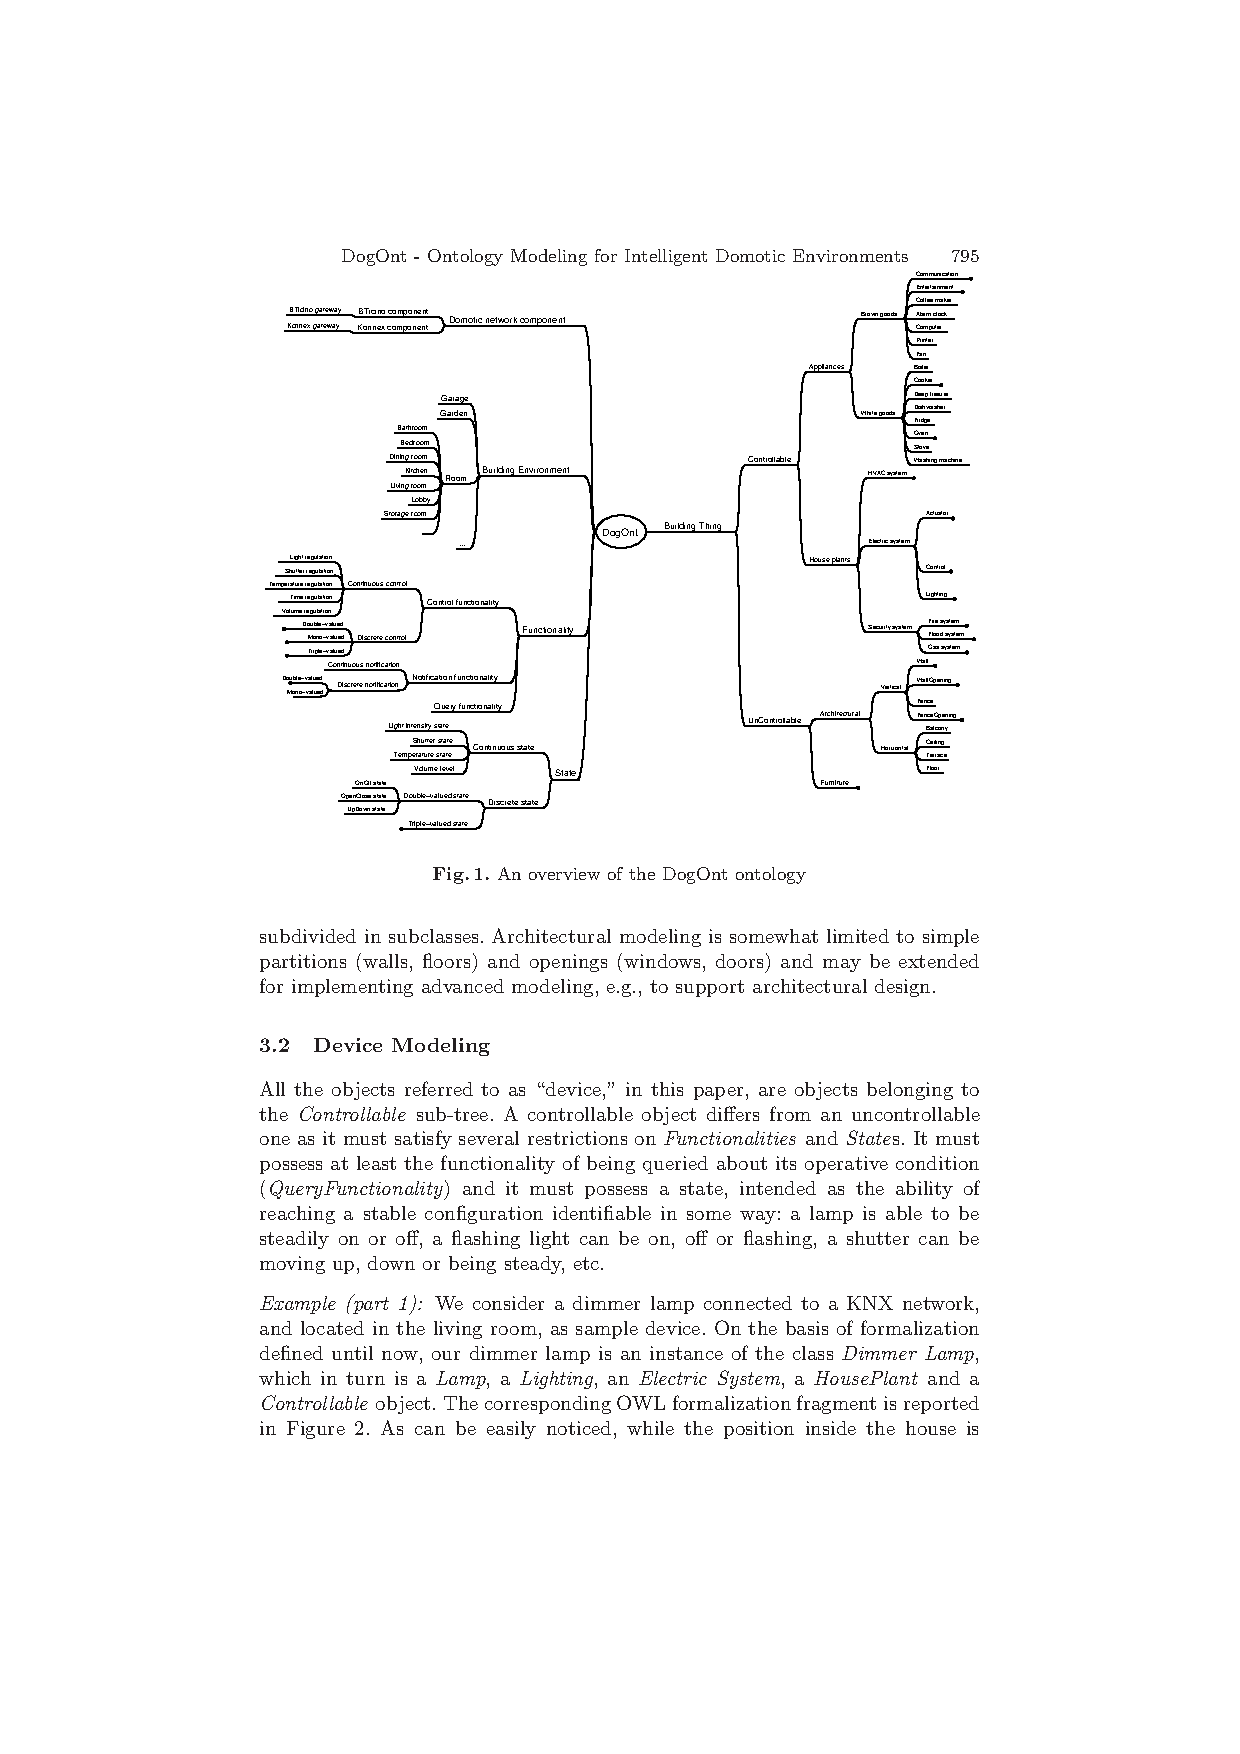
\includegraphics[width=0.9\textwidth, trim=4cm 15.5cm 4cm 4.6cm, clip]{rw-supervision-dogont}
    \caption{L'ontologie de DogOnt}\label{fig:rw:supervision:dogont}
\end{figure}

Plusieurs autres projets ont permit ce type de modélisation pour des applications pervasives. Par exemple, Amigo~\cite{BenMokhtar:easy} se focalise plus sur la modélisation des services et des capacités. A contrario, \textit{MATCH}~\cite{Docherty:match} met l'accent sur la hiérarchie des ontologies pour que chaque domaine puisse apporter ses connaissances en se raccrochant à des concepts communs (\textit{dispositifs}, \textit{réseau},\dots).

Ces projets appliquent les idées de \textit{CIM} (détaillé en section~\ref{sec:rw:supervision:administration}) en tentant de représenter toutes les possibilités de données dans leurs cadres applicatifs respectifs. Le concept le plus haut étant \textit{Controllable} pour ensuite en dériver les autres classes. Le point important étan que pour intégrer toutes les sources de données, elles doivent donc respecter ce grand ensemble de classes. Cependant, dans le domaine des ontologies, les standards de modélisations n'existent pas, notamment pour des domaines en particulier. Bien heureusement, 

\subsubsection{SOCAM : De l'utilité du raisonnement logique}
SOCAM (Service-Oriented Context-Aware Middleware)~\cite{Gu:socam} propose un intergiciel générique pour permettre aux développeurs de créer des applications pervasives par contexte. Cet intergiciel supporte l'acquisition, la découverte, l'interprétation et l'accès aux contextes. Comme les autres solutions présentés jusqu'ici, il s'appuie sur une ontologie conceptualisée comme celle de \textit{MATCH} afin de pouvoir être générique et y apporter les connaissances de chacun des domaines.

L'architecture de SOCAM, représentée en figure~\ref{fig:rw:supervision:socam} qui se décrit en trois 4 composants principaux.
\begin{figure}[ht]
    \centering
    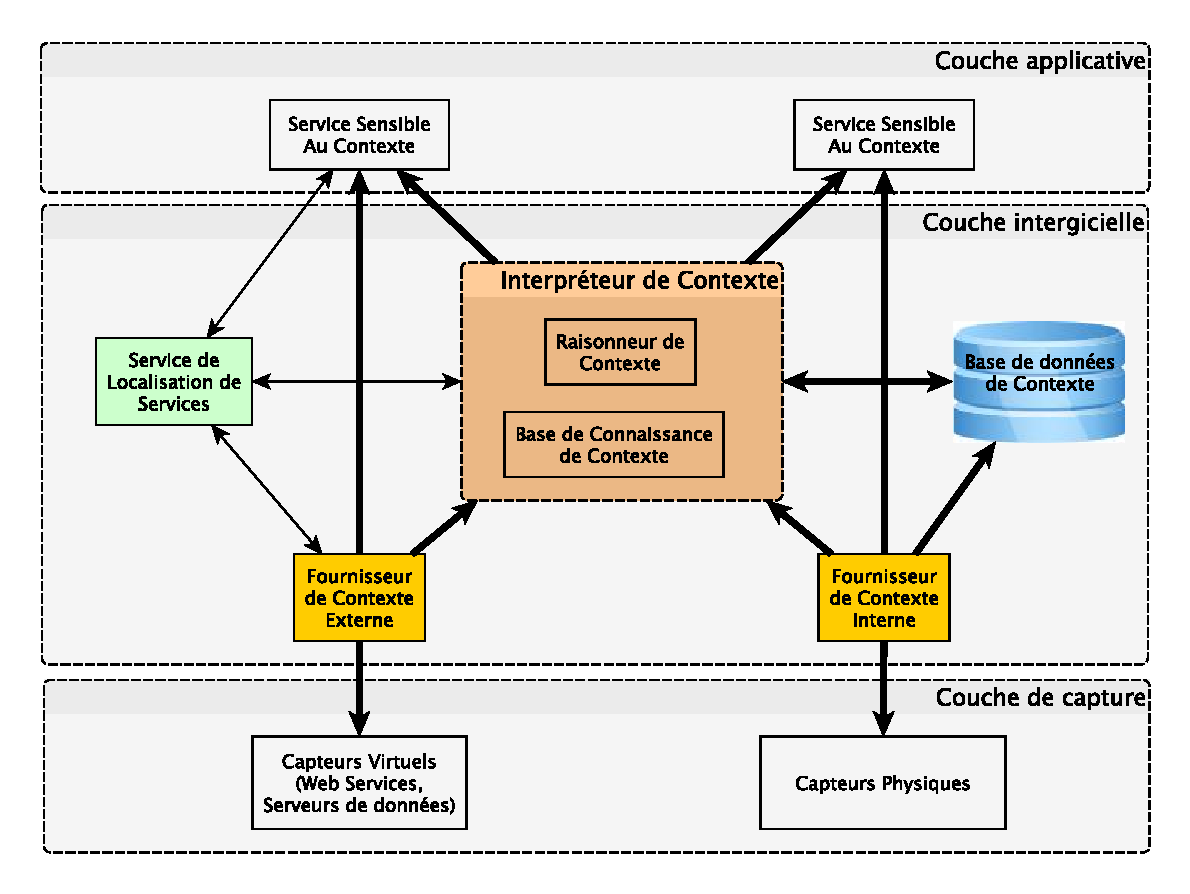
\includegraphics[width=0.75\textwidth]{rw-supervision-socam}
    \caption{Architecture de SOCAM}\label{fig:rw:supervision:socam}
\end{figure}
\begin{itemize}
	\item[\textbf{Fournisseurs de contexte}] Ceci permet d'abstraire l'hétérogénéité des données issues des différentes sources (internes, tels que les capteurs ou devices), ou externe (services méteo ou autres) pour les convertir en \textit{OWL}. Les données insérés doivent être du plus haut niveau possible. Par exemple, dans un fournisseur de données à partir de vidéo, il est plus pertinent d'insérer les données traités telles que \enquote{\it la personne est allongée sur le lit} ou \enquote{\it un intrus est dans la maison}. Ainsi, les définitions de règles et leurs inférences se concentrent sur le processus métier de l'analyse contextuelle et non sur l'abstraction sémantique des informations.
    \item[\textbf{Interpréteur de contexte}] Fournit la logique de raisonnement sur le contexte.
    \item[\textbf{Base de données de contexte}] Stocke les ontologies de contexte et l'historique des contextes pour chaque sous-domaine.
    \item[\textbf{Service de localisation de services}] Sert de catalogue des services externes disponibles. Son filtrage peut se faire sur un type de service mais il peut aussi faire une comparaison sur le contexte que le service fournit. Par exemple, si l'application souhaite \verb|(John socam:locatedIn ?x)|, alors le localisateur va chercher sur les instances de contextes pour voir qui peut lui fournir ce genre de données~\cite{}.
\end{itemize}
Les services applicatifs utilisant la notion de contexte, vont ainsi utiliser les fonctionalitées que fournits SOCAM pour gérer cet ensemble de données. Une manière classique de construire ces services étant de spécifier des actions déclenchés par un ensemble de règles au moment où le contexte change.

SOCAM implémente deux manières de faire de l'inférence logique de prédicats. La première étant l'inférence structurelle. En effet, l'application d'une propriété transitive à un concept nous donne plusieurs informations. 

Par exemple si nous avons que \verb|(John socam:locatedIn socam:Kitchen)| et que \verb|(Kitchen socam:locatedIn socam:FirstFloor)|, alors étant donnée que \verb|(socam:locatedIn rdf:type owl:TransitiveProperty)|, le langage de l'ontologie sous-jacente (\textit{OWL/Lite}) indique que \verb|(John socam:locatedIn socam:FirstFloor)|.

La deuxième manière, toutefois similaire, est un ensemble de règles utilisateurs. En utilisant un moteur similaire aux moteurs \textit{Prolog}, il est possible d'induire des prédicats applicatifs. En exemple, les auteurs nous donnent par exemple :
\begin{verbatim}
    (?user rdf:type socam:Person)
    (?user socam:locatedIn socam:Bedroom)
    (?user socam:hasPosture 'LIEDOWN')
    (socam:Bedroom socam:lightLevel 'LOW')
    (socam:Bedroom socam:doorStatus 'CLOSED')
            => (?user socam:status 'SLEEPING')
\end{verbatim}

Il est important de noter que d'un point de vue performance, l'ordre de grandeur est au alentour de la seconde pour faire le traitement d'une règle sur une machine de faible performances. La complexité du traitement des requêtes d'inférence est \textit{PSPACE} et celle du langage de l'ontologie est de \textit{EXPTIME}. Ce qui fait que la montée en taille de la base de connaissance rendra plus difficile son exécution.
\subsection{Synthèse}
\TODO{Et c'est reparti pour le tableau}